\documentclass[a4paper,12pt]{article}

\usepackage[ngerman]{babel}
\usepackage{amsmath}
\usepackage{amssymb}
\usepackage{graphicx}
\usepackage[a4paper,margin=2cm]{geometry}
\usepackage{float}
\usepackage{enumitem}
\title{Ladung und Potential}
\author{}
\date{}

\begin{document}
    
    \maketitle
    \tableofcontents
    
    \section{Ladung und Potential}
    
    \subsection{Ladung}
    Die elektrische Ladung ist eine Erhaltungsgrösse. Kann nicht erzeugt oder vernichtet werden, nur umverteilt.
    
    Formelzeichen: $Q$
    
    Einheit: $C$ – $As$ – Coulomb
    
    $$Q = I \cdot t$$
    
    \subsubsection{Elementare Ladung}
    Proton $+e$ Elektron $-e.$
    $$e = 1.6 \cdot 10^{-19}$$
    $$[e] = As - Amperesekunden$$
    
    \subsubsection{Elektronen entnehmen}
    Wie viele Elektronen können aus einer Ladung entnommen werden?
    $$N_e = \frac{Q}{e}$$
    
    \subsubsection{Wie viele Atome in Eisen}
    Dichte von Eisen $7.8\frac{g}{cm^3}$
    
    1 Mol Eisen $\approx 6.022 \cdot 10^{23}$ Atome $\approx 58.8g$
    
    $1cm^3$ Eisen: $\approx 7.8g \approx 0.14 Mol$
    $$N_{Fe} = 0.14 \cdot 6.022\cdot10^{23} = 8.4 \cdot 10^{22}$$
    Atome pro Kubikmeter:
    $$n_{Fe}=8.4\cdot10^{22}\,cm^{-3}$$
    
    \subsubsection{Beispiel Ladung Batterie}
    %\includegraphics[width=0.5\textwidth]{9a7509862a07413de46f34c98c7a5a64.png}
    
    \subsection{Elektrische Energie}
    $$W = Q U$$
    
    \subsection{Strom- und Ladungsdichte}
    
    \subsubsection{Strom}
    Elektrischer Strom ist die Ladung, die sich pro Zeit durch einen Leiter bewegt.
    $$I = \frac{\Delta Q}{\Delta t}$$
    $$[I] = \frac{As}{s} = A$$
    
    \subsubsection{Stromdichte (Strom pro Fläche)}
    Die Stromdichte beschreibt den Zusammenhang:
    $$J = \frac{|I|}{A} = n q v_D = \rho v_D$$
    
    Ladungsträger pro Volumeneinheit:
    $$[n] = \frac{1}{m^3}$$
    
    Ladung eines Teilchens:
    $$[q] = As$$
    
    Driftgeschwindigkeit:
    $$[v_D] = \frac{m}{s}$$
    
    Stromdichte:
    $$J = \frac{A}{m^2}$$
    
    \subsubsection{Ladungsdichte (Ladung pro Volumen)}
    Will man wissen, wie viel Ladung sich in einem Volumen befindet, so spricht man von der \textbf{Ladungsdichte} oder auch \textit{Volumenladungsdichte}, abgekürzt mit $\rho$. Achtung, nicht zu verwechseln mit dem spezifischen Widerstand, der ebenfalls das Formelzeichen $\rho$ hat.
    
    $$\rho = n \cdot e$$
    $$\rho = \frac{\Delta Q}{\Delta V}$$
    $$\rho = \frac{R \cdot A}{L}$$
    
    \subsection{Ohmscher Widerstand}
    Elektrische Widerstand und Leitwert
    
    Der elektrische Widerstand lässt sich aus dem Ohmschen Gesetz berechnen:
    $$R = \frac{U}{I}$$
    
    Der Widerstand lässt sich alternativ auch aus der Länge, der Fläche und dem spezifischen Widerstand des Materials berechnen:
    $$R = \frac{\rho \cdot l}{A}$$
    
    Der elektrische Leitwert ist das Reziproke des Widerstands:
    $$G = \frac{1}{R}$$
    $$G = \frac{l}{\kappa \cdot A} = \frac{A}{\rho \cdot l}$$
    
    $$[G] = S \text{ (Siemens)}$$
    
    \subsubsection{Spezifischer Leitwert und spezifischer Widerstand}
    Wie bereits gesehen, existiert für jedes Material ein spezifischer Widerstand $\rho$.
    $$\rho = \text{spezifischer Widerstand}$$
    
    Das Reziproke des spezifischen Widerstands ist der spezifische Leitwert $\kappa$ oder $\sigma$:
    $$\kappa = \frac{1}{\rho}$$
    
    \subsubsection{Veränderung des Widerstands bei verschiedener Temperatur}
    Der elektrische Widerstand von Materialien kann sich bei verschiedener Temperatur verändern. Meistens wird der Widerstand bei grösserer Temperatur auch grösser. Das liegt daran, dass die Atome sich mehr bewegen und Kollisionen dadurch häufiger werden.
    
    $$\rho(T)=\rho_{20}[1+\alpha_{20}(T-293K)]$$
    gilt auch für gesamte Widerstände:
    $$R(T)=R_{20}[1+\alpha_{20}(T-293K)]$$
    
    \textbf{Hinweis:} Absoluter Nullpunkt $-273.15^\circ C$, $20^\circ C = 293K$
    
    Beispiel:  
    Eisen erhitzt sich auf $303K$ also $30^\circ C$:
    $$R_{20} = 100 \Omega$$
    $$\alpha_{20Fe}=6.5\cdot 10^{-3}K^{-1}$$
    $$R_{Fe}(303)=100[1+6.5\cdot10^{-3}(10)] = 103.8 \Omega$$
    
    \section{Formelsammlung Gleichstrom}
    
    \subsection{Ohmsches Gesetz}
    $$U=R\cdot I$$
    $$R=\frac{U}{I}$$
    $$I=\frac{U}{R}$$
    
    $$[U]=V - Volt$$
    $$[R]=\Omega - Ohm$$
    $$[I]=A - Ampere$$
    
    \subsubsection{Potentialform ohmsches Gesetz}
    Betrachtet man das ohmsche Gesetz für genau einen Widerstand, entspricht $U$ der Spannung,
    welche über dem Widerstand abfällt. Das lässt sich auch als Differenz vom Potential
    „über“ und „unter“ dem Widerstand darstellen.
    $$I = \frac{U_{oben}-U_{unten}}{R}$$
    
    Diese Form ist v.a. hilfreich, wenn man das KCL (Kirchhoff Current Law) anwendet.
    
    \subsection{Elektrische Leistung}
    $$P=U\cdot I=\frac{U^2}{R}=I^2R$$
    
    $$[P]=W - Watt$$
    $$[U]=V - Volt$$
    $$[I]=A - Ampere$$
    
    \subsection{Zählpfeilsystem}
    
    \subsubsection{Erzeugerzählpfeilsystem (EZS)}
    Wenn positiv wird Leistung abgegeben:
    $$U=-R\cdot I$$
    %\includegraphics[width=0.5\textwidth]{a8822bf910fa46d5b6b30c551868eb20.png}
    
    \subsubsection{Verbraucherzählsystem (VZS)}
    Wenn positiv wird Leistung aufgenommen:
    $$U=R\cdot I$$
    %\includegraphics[width=0.5\textwidth]{5a20a3573a714196af44b2bb9619b833.png}
    
    \subsection{Aktive Zweipole}
    
    \subsubsection{Reale Spannungsquelle}
    $$U=U_0-I\cdot R_i$$
    $$R_i=\frac{U}{I}$$
    $$R_i=\frac{U_0}{I_k}$$
    %\includegraphics[width=0.6\textwidth]{ad1caf2eb13c48da9e53e1d271f661be.png}
    
    \subsubsection{Reale Stromquelle}
    $$I=I_0-\frac{U}{R_i}$$
    %\includegraphics[width=0.6\textwidth]{63f6d13ca1ef4554951310502705f5a7.png}
    
    \subsection{Kirchhoffsche Gesetze}
    
    \subsubsection{Knotensatz (1.)}
    $$\sum_{k=1}^n I_k = 0$$
    \begin{figure}[H]
        \centering
        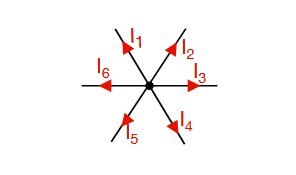
\includegraphics[width=0.6\textwidth]{img/knotensatz.png} % your file name
        \caption{My image caption}
        \label{fig:meinbild32}
    \end{figure}
    
    $$I_1+I_2+I_3-I_4=0$$
    
    \paragraph{Knotengleichungen aufstellen}
    TBD
    
    \subsubsection{Maschensatz (2.)}
    $$\sum_{k=1}^n U_k = 0$$
    \begin{figure}[H]
        \centering
        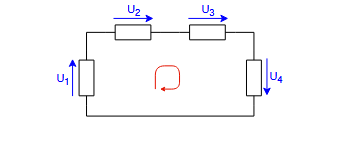
\includegraphics[width=0.6\textwidth]{img/maschensatz.png} % your file name
        \caption{My image caption}
        \label{fig:meinbild32}
    \end{figure}
    
    $$-U_5+U_4-U_3+U_2-U_1=0$$
    
    \paragraph{Maschengleichungen aufstellen}
    TBD
    
    \subsection{Serienschaltung von Widerständen (Spannungsteiler)}
    $$R_{ers}=\sum_{k=1}^n R_k$$
    $$U=I(R_1+R_2+\dots+R_n)=I\tilde{R}$$
    
    \subsubsection{Spannungsteiler}
    $$\frac{U_1}{U}=\frac{R_1}{R_{ers}}$$
    
    \subsection{Parallelschaltung von Widerständen}
    $$G_{ers}=\sum_{k=1}^n G_k$$
    $$U=I\cdot\frac{1}{G_1+G_2+\dots+G_n}$$
    
    \subsubsection{Parallelschaltung von zwei Widerständen}
    $$R_{12}=\frac{R_1R_2}{R_1+R_2}$$
    
    \subsubsection{Stromteiler}
    $$\frac{I_1}{I_{ges}}=\frac{G_1}{G_{sum}}$$
    $$I_1=I\frac{G_2}{G_1+G_2}$$
    $$I_2=I\frac{G_1}{G_1+G_2}$$
    
    \subsection{Stern- und Dreieckschaltung}
    \begin{figure}[h!]
        \centering
        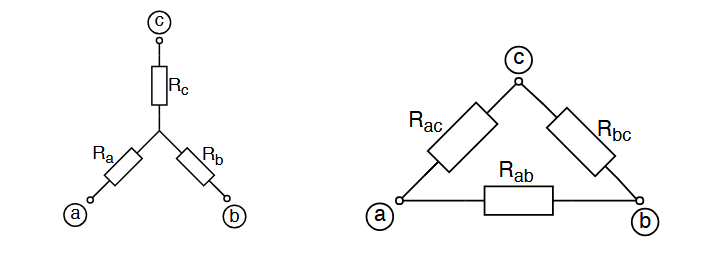
\includegraphics[width=0.6\textwidth]{img/stern_dreieck.png} % your file name
        \caption{My image caption}
        \label{fig:meinbild2}
    \end{figure}
    
    \subsubsection{Stern $\rightarrow$ Dreieck}
    $$\tilde{R}=R_aR_b+R_aR_c+R_bR_c$$
    $$R_{ab}=\frac{\tilde{R}}{R_c}$$
    $$R_{ac}=\frac{\tilde{R}}{R_b}$$
    $$R_{bc}=\frac{\tilde{R}}{R_a}$$
    
    \subsubsection{Dreieck $\rightarrow$ Stern}
    $$\hat{R}=R_{ab}+R_{ac}+R_{bc}$$
    $$R_a=\frac{R_{ab}R_{ac}}{\hat{R}}$$
    $$R_b=\frac{R_{ab}R_{bc}}{\hat{R}}$$
    $$R_c=\frac{R_{ac}R_{bc}}{\hat{R}}$$
    
    \subsection{Leistungsanpassung}
    $$R_i = R_L$$
    $$\eta = \frac{R_i}{R_i+R_L} = 50\%$$
    $$I=\frac{U_0}{2R_i}$$
    $$P_{max}=\frac{U_0^2}{4R_i}$$
    \begin{figure}[h!]
        \centering
        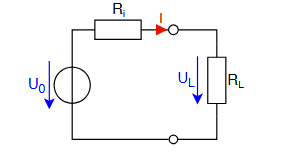
\includegraphics[width=0.6\textwidth]{img/leistungsanpassung.png} % your file name
        \caption{My image caption}
        \label{fig:meinbil2}
    \end{figure}
    
    \subsection{Messen elektrischer Grössen}
    Für $RA = 10 \Omega$ und $RV = 10 M\Omega$ gilt $RL = 10 k\Omega$. Widerstände unter $10 k\Omega$ sollten daher spannungsrichtig
    gemessen werden
    \subsubsection{Bestimmung von Messefehler}
    $$I=\frac{U_0}{R_i+R_L}$$
    $$I_M=\frac{U_0}{R_i+R_L+R_A}$$
    $$\Delta I = I_M - I$$
    $$\delta I = \frac{\Delta I}{I}$$
    
    \subsubsection{Stromrichtige Messung}
    $$I_M=I_L$$
    $$U_M=I_M(R_A+R_L)$$
    \begin{figure}[H]
        \centering
        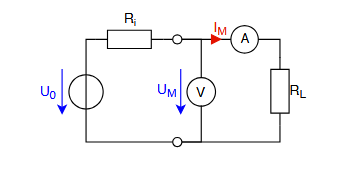
\includegraphics[width=0.6\textwidth]{img/messung_stromrichtig.png} % your file name
        \caption{My image caption}
        \label{fig:meinbild}
    \end{figure}
    
    \subsubsection{Spannungsrichtige Messung}
    $$U_M=U_L$$
    $$I_M=I_L+\frac{U_M}{R_V}$$
    \begin{figure}[H]
        \centering
        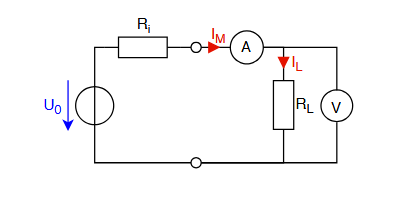
\includegraphics[width=0.6\textwidth]{img/messung_spannungsrichtig.png} % your file name
        \caption{My image caption}
        \label{fig:meinbild1}
    \end{figure}
    
    \section{Superposition}
    Beim Supoerpositionsverfahren kann jeder Spannungs oder Stromquelle einzeln betrachtet werden. Dazu werden jeweils alle nicht betrachteten Quelle folgendermassen ersetzt:
    
    \begin{itemize}
        \item Spannungsquelle wird zu Kurzschluss
        \item Stromquelle wird zu Leerlauf
    \end{itemize}
    
    \begin{figure}[H]
        \centering
        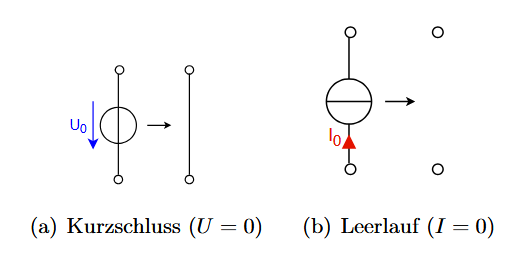
\includegraphics[width=0.6\textwidth]{img/superposition.png} % your file name
        \caption{My image caption}
        \label{fig:meinbild1}
    \end{figure}
    
    \subsection{geschlossen Netzwerk}
    Vorgehen bei einem geschlossenen Netzwerk:
    \begin{enumerate}
        \item Alle Quellen einzeln betrachten und die Teilspannung und Ströme berechnen.
        \item Vorzeichen anhand der Stromflussrichtung beachten
        \item Teilströme- und Spannungen zusammenrechnen
    \end{enumerate}
    
    \subsection{offenes Netzwerk (offene klammern)}
    Sind die klemmen offen und soll die Spannung und Strom an den Klemmen bestummen werden geht man wie folge vor:
    
    \begin{enumerate}
        \item Superposition anwenden, Quellen isolieren.
        \item Um die Spannung an der Quellen zu bestimmen, lässt man die Quellen offen und bestimmt das Potenzial am letzten punkt vor der Klemme.
        \item  Um den Strom zu bestimmen schliesst man die Klemmen kurz. Jetzt kann man alle Widerstände streichen durch die wegen dem Kurzschluss kein strom fliesst.
        \item Vorzeichen anhand der Stromflussrichtung beachten
        \item Teilströme- und Spannungen zusammenrechnen
    \end{enumerate}
    
    \section{Zweipolersatzschaltung}
    Bei offenen Klemmen git: \\
    innenwiderstand $R_i$, Quellespannung $U_q$, Kurzschlussstrom $I_k$
    $$R_i=\frac{U_q}{I_k}$$
    
    \subsection{Thévenin}
    
    Jedes lineare Zweipol-Netzwerk kann ersetzt werden durch
    eine ideale Spannungsquelle $U_{\text{th}}$ in Serie mit einem Widerstand $R_{\text{th}}$.
    
    \[
    U_{\text{th}} = \text{Leerlaufspannung}
    \]
    \[
    R_{\text{th}} = \text{Widerstand bei deaktivierten Quellen}
    \]
    
    \vspace{1em}
    
    
    \subsection{Norton}
    
    Dasselbe Netzwerk kann ersetzt werden durch
    eine ideale Stromquelle $I_{\text{n}}$ parallel zu einem Widerstand $R_{\text{n}}$.
    
    \[
    I_{\text{n}} = \text{Kurzschlussstrom}
    \]
    \[
    R_{\text{n}} = R_{\text{th}}
    \]
    
    \vspace{1em}
    
    \section{Wheatstone}
    \subsection{hochohmiges Voltmeter}
    Bei offenen Klemmen kann maneinfach den Spannungsteiler benutzten. Der Widerstand zwischen den Klemmen ist quasi $\infty$ gross.
    \\
    
    links:
    $$U_A=U_0*\frac{R2}{R1+R2}$$
    
    rechts:
    $$U_B=U_0*\frac{R4}{R3+R4}$$
    
    Klemmspannung:
    $$U_{AB}=U_A - U_B$$
    \begin{figure}[H]
        \centering
        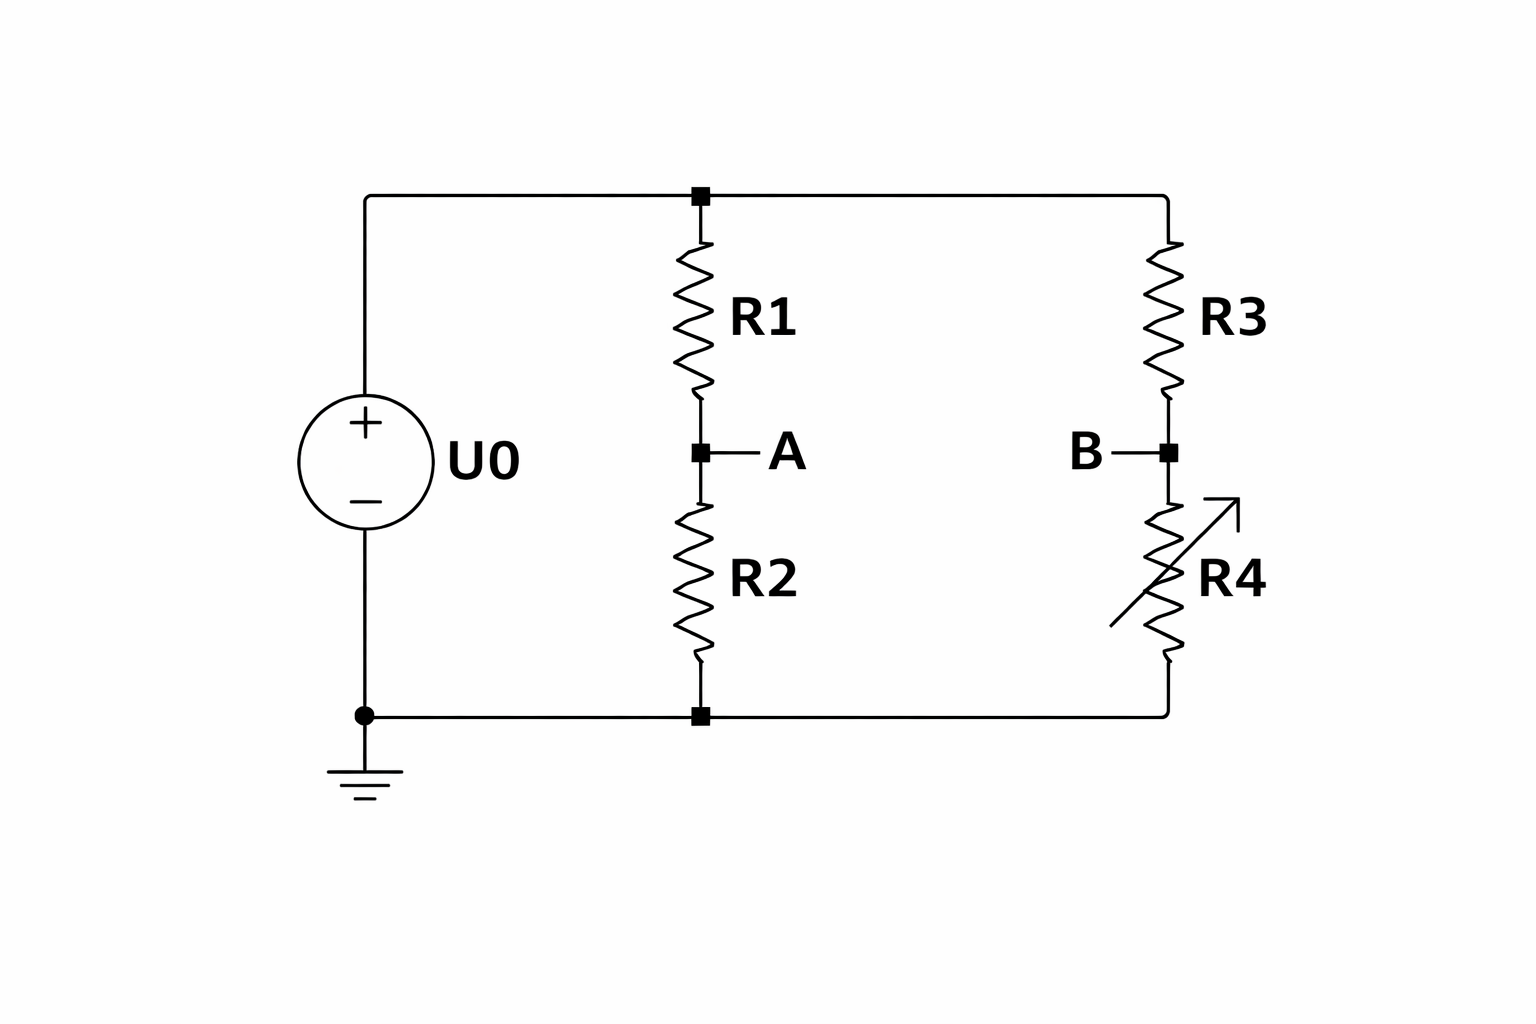
\includegraphics[width=0.6\linewidth]{img/wheatstone_high_resitance.png} % your file name
        \caption{My image caption}
        \label{fig:meinbild14}
    \end{figure}
    
    \pagebreak
    
    \subsubsection{Voll- und Halbbrücke}
    Die Wheatstonebrücke kann entweder mit 4 oder 2 Sensoren betrieben werden. Je nach dem verändert sich die emfpindlichkeit der Brücke:
    
    \paragraph{Halbbrücke}\mbox{}\\
    \begin{figure}[H]
        \centering
        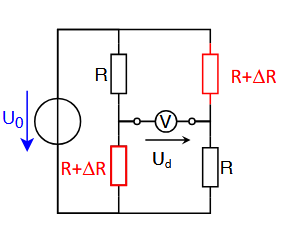
\includegraphics[width=0.4\linewidth]{img/halbbrücke.png} % your file name
        \caption{Halbbrücke}
        \label{fig:halbbr}
    \end{figure}
    
    $$U_d\approx\frac{U_0}{2}\frac{\Delta R}{R}$$
    
    \paragraph{Vollbrücke}\mbox{}\\
    \begin{figure}[H]
        \centering
        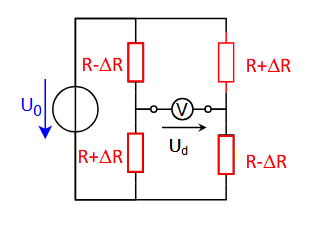
\includegraphics[width=0.4\linewidth]{img/vollbrücke.png} % your file name
        \caption{Vollbrücke}
        \label{fig:vollbr}
    \end{figure}
    
    
    $$U_d\approx{U_0}\frac{\Delta R}{R}$$
    
    \pagebreak
    
    \subsection{elektronische Messschaltung}
    Setzten man nun einen Widerstand zwischen den klemmen ein verändert sich die Spannung. Für einen unendlich grossen Widerstand ist Spannung gliech $U_AB$. Setzt man einen Widerstand ein, so muss für die neue Spannung gelten $U_{Rm} < U_{AB}$. Dazu berechnen wir zuerst denn Innenwiderstand der Brückenschaltung und danach über denn Spannungsteiler die effketive Spannung $U_{Rm}$
    \\
    
    Innenwiderstand:
    $$R_i = (R1||R2)+(R3||R4) = \frac{R1*R2}{R1+R2}+\frac{R3*R4}{R3+R4}$$
    
    Spannung über Rm:
    $$U_{R_m}=U_{AB}*\frac{R_m}{R_i+R_m}$$
    
    
    \begin{figure}[H]
        \centering
        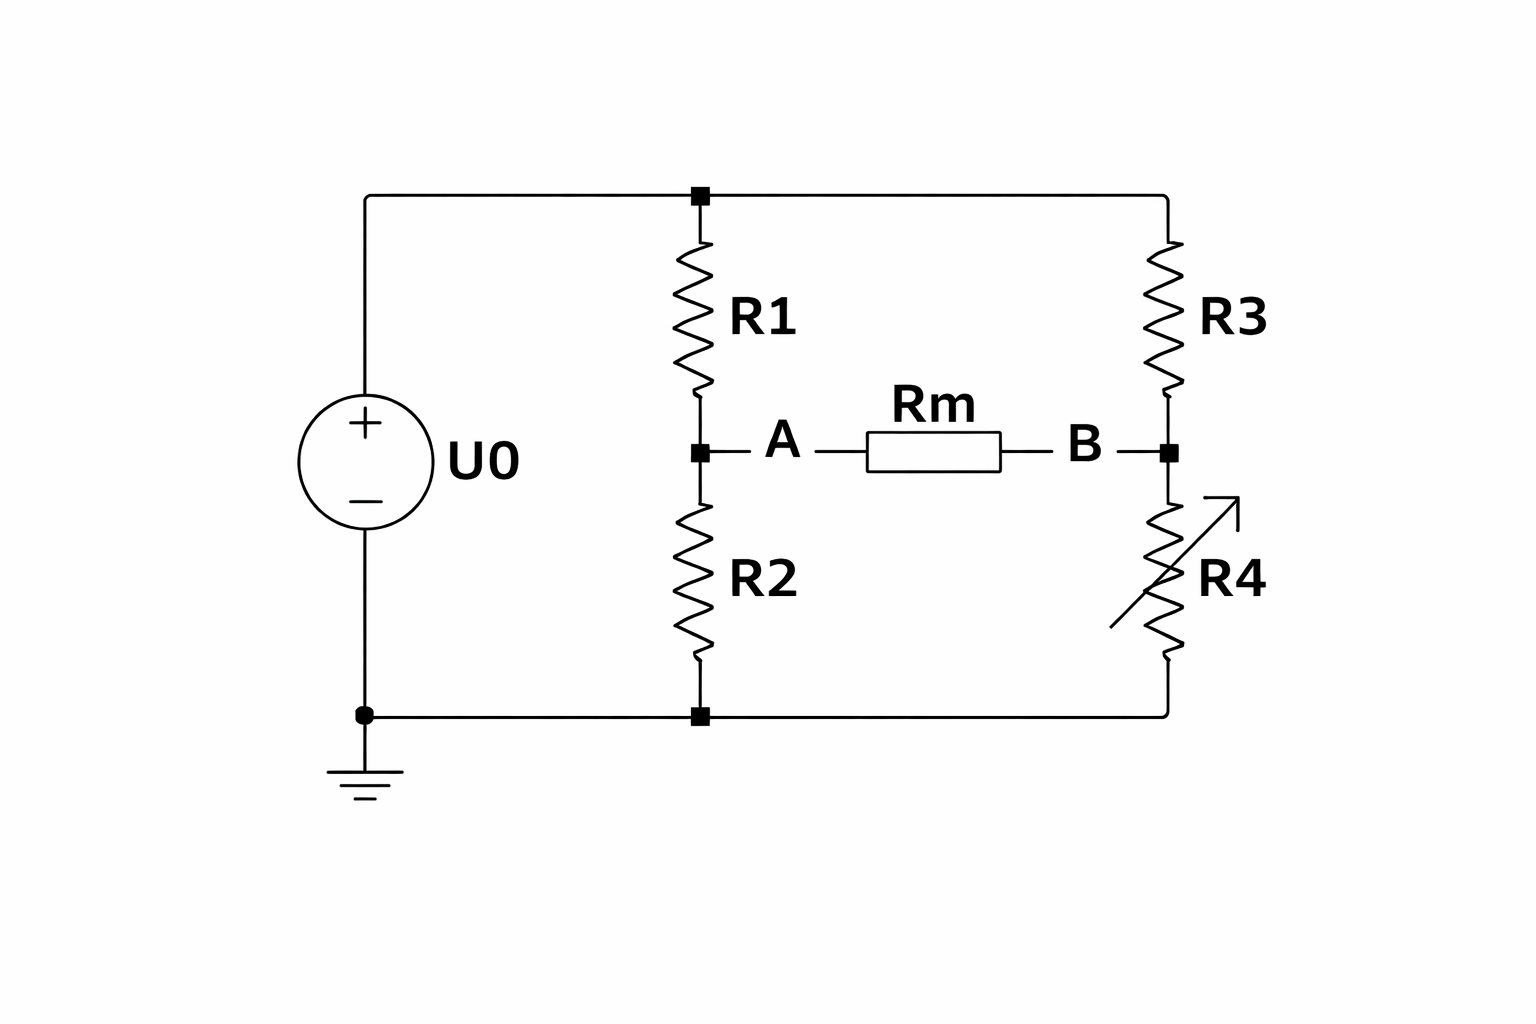
\includegraphics[width=0.6\textwidth]{img/wheatstone_electric_meassurement.png} % your file name
        \caption{My image caption}
        \label{fig:meinbild13}
    \end{figure}
    
    Ist die Spannung $U_{Rm}$ bekkant können die neuen Spannung über $R1 .. R4$ über den Kontensatz bestummen werden:
    \\
    
    \textbf{Knotengleichungen:}
    
    Gleichungsystem mit 2 Gleichungen und 2 unbekannten. Nach $U_A$ oder $U_B$ auflösen und einsetzten.
    \begin{align}
        \frac{U_A-10}{R_1}+\frac{U_A}{R_2}+\frac{U_A-U_B}{R_m} &= 0 \\
        \frac{U_B-10}{R_3}+\frac{U_B}{R_4}+\frac{U_B-U_A}{R_m} &= 0
    \end{align}
    
    
    \textbf{Spannungsabfälle:}
    \[
    U_{R1}=10-U_A,\quad
    U_{R2}=U_A,\quad
    U_{R3}=10-U_B,\quad
    U_{R4}=U_B
    \]
    
    \pagebreak
    
    \section{Kondensator}
    Kondensator kann wie eine Offen Klemme behandelt werden.
    \subsection{Ladung}
    $$Q = C \cdot U$$
    
    \subsection{Spannung}
    $$U = \frac{Q}{C}$$
    
    \subsection{Kapazität}
    $$C = \frac{Q}{U}$$
    
    Plattenkondensator:
    $$C = \varepsilon_0 \cdot \frac{A}{d}$$
    
    \subsection{gespeicherte elektrische Energie}
    $$W = \frac{1}{2} C U_0^2$$
    
    \subsection{Parallelschaltung}
    Bei der Parallelschaltung von Kondesatorn adddiert sich die Kapzitäten. (Analog Sereinschaltung Widerstände)
    $$C_p = \sum C_i$$
    
    \subsection{Serienschaltung}
    Bei der Serineschaltung addieren sich die Kerhwerte (analog Paralellschaltung Widerstand):
    $$\frac{1}{C_s} = \sum \frac{1}{C_i}$$
    
    \subsection{Laden und Entladen eines Kondensators}
    
    \subsubsection*{Laden eines Kondensators (RC-Reihenschaltung)}
    
    Maximale Spannung in einer Schaltung, Konten vor und nach Kondensator:
    \[
    u_C(t)=U_{links}(t) - U_{rechts}(t)
    \]

    Spannung am Kondensator über Zeit:
    \[
    u_C(t)=U_0\left(1-e^{-\frac{t}{\tau}}\right)
    \]
    
    \begin{figure}[H]
        \centering
        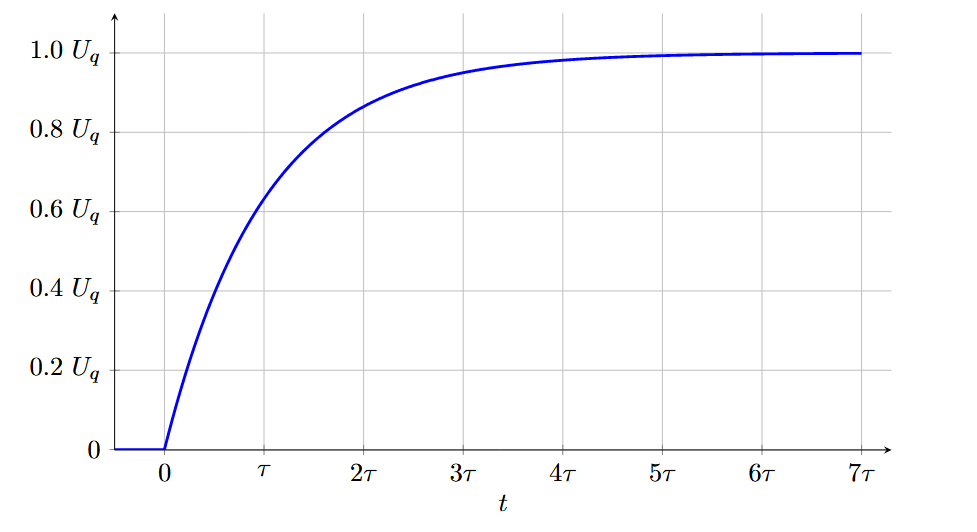
\includegraphics[width=0.6\textwidth]{img/kodensator_laden_spannung.png} % your file name
        \caption{My image caption}
        \label{fig:meinbild1311}
    \end{figure}
    
    Strom:
    \[
    i(t)=\frac{U_0}{R}\,e^{-\frac{t}{RC}}
    \]
    
    \begin{figure}[H]
        \centering
        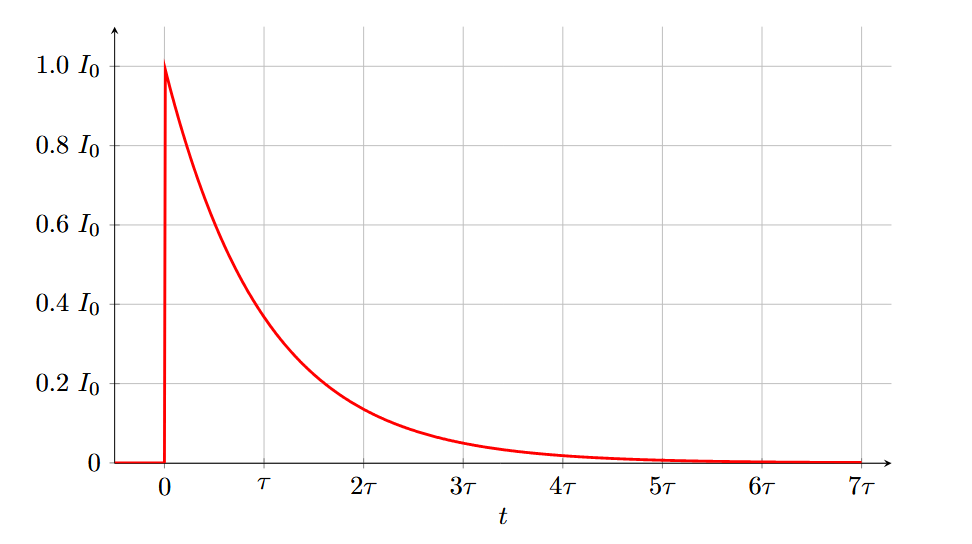
\includegraphics[width=0.6\textwidth]{img/kodensator_laden_strom.png} % your file name
        \caption{My image caption}
        \label{fig:meinbild132}
    \end{figure}
    
    \subsubsection*{Entladen eines Kondensators}
    Spannung:
    \[
    u_C(t)=U_0\,e^{-\frac{t}{RC}}
    \]
    
    \begin{figure}[H]
        \centering
        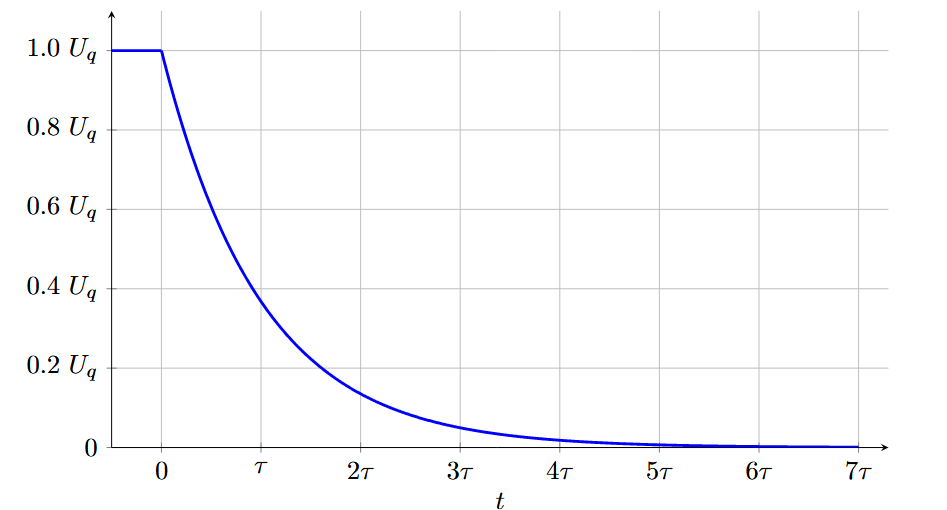
\includegraphics[width=0.6\textwidth]{img/kodensator_entladen_spannung.png} % your file name
        \caption{My image caption}
        \label{fig:meinbild134}
    \end{figure}
    
    Strom:
    \[
    i(t)=-\frac{U_0}{R}\,e^{-\frac{t}{RC}}
    \]
    
    \begin{figure}[H]
        \centering
        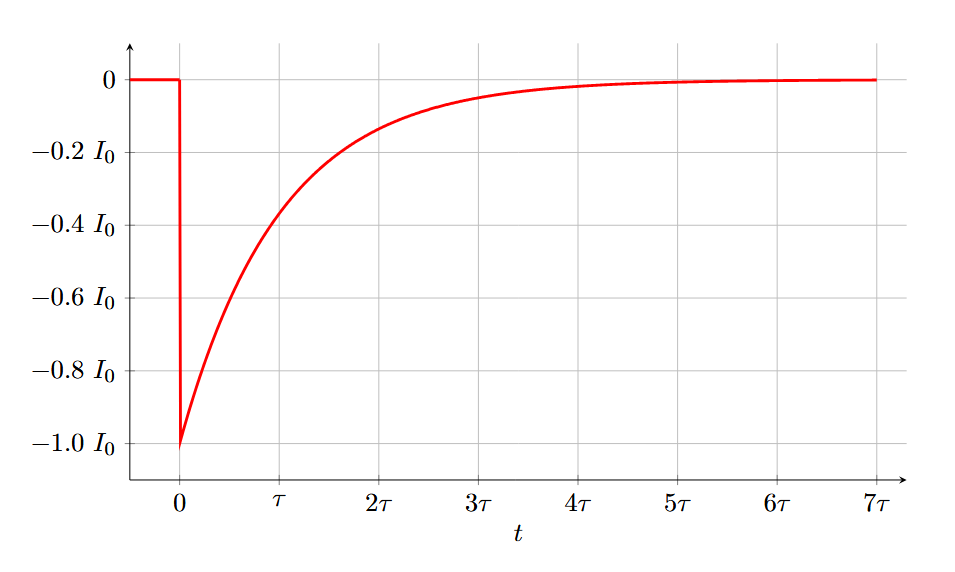
\includegraphics[width=0.6\textwidth]{img/kodensator_entladen_strom.png} % your file name
        \caption{My image caption}
        \label{fig:meinbild1345}
    \end{figure}
    
    \subsubsection*{Zeitkonstante \(\tau\)}
    \[
    \tau = R \cdot C
    \]
    
    Einheit:
    \[
    [\tau] = \mathrm{s}
    \]
    
    Nach einer Zeitspanne \(\tau\):
    \[
    u_C(\tau) \approx 0.63\,U_0 \quad (\text{beim Laden})
    \]
    \[
    u_C(\tau) \approx 0.37\,U_0 \quad (\text{beim Entladen})
    \]
    
    Nach etwa \(5\tau\) gilt der Kondensator praktisch als vollständig geladen bzw. entladen
    (\(>99\%\)).
    
    \section{elekt. Bauteile}
    \subsection{z-Diode}
    \begin{minipage}[t]{0.5\columnwidth}
        \begin{itemize}[label={}, leftmargin=*,  itemsep=0.1em]
            \item \textbf{Zener-Effekt}: \\ bei geringer Spannung $\rightarrow U < 5V$
            \item \textbf{Arbeitspunkt}: \\ nicht lineare Bauteil! \\ \\ Spannung,Strom,Widerstand kann nicht ber ohmsches Gesetzte berechnet werden \\  \\ immer über \textbf{Maschengeleichung!}
        \end{itemize}
    \end{minipage}\hfill
    \begin{minipage}[t]{0.5\columnwidth}
        \begin{itemize}[label={}, leftmargin=*]
            \item \textbf{Avalanche-Effekt}: \\ bei grösseren Spannungen $\rightarrow U > 5V$
            \item \textbf{Leistung}: \\  nicht lineare Bauteil! \\ \\ Komponetnen werden separat behandelt \\ \\ $P_z = P_{rz} + P_{Uz}$
        \end{itemize}
    \end{minipage}\hfill
    
\end{document}
